\documentclass[10pt]{developercv}
\usepackage{multicol}
\setlength{\columnsep}{0mm}
\usepackage{lipsum}  
\usepackage{graphicx}

\begin{document}
\begin{minipage}[t]{0.4\textwidth} 
	\vspace{-\baselineskip}
	\vspace{5pt}

	{ \fontsize{18}{20} \textcolor{black}{\textbf{\MakeUppercase{Lavrushchev Ivan}}}}
	
	\vspace{8pt}

    {\Large Student $\sim$ Developer}
\end{minipage}
\begin{minipage}[t]{0.23\textwidth}
	\vspace{-\baselineskip}
	
    \icon{Github}{11}{\href{https://github.com/livlavr}{github.com/livlavr}}\\
    \icon{Gitlab}{11}{\href{https://gitlab.com/livlavr}{gitlab.com/livlavr}}\\
    \icon{MapMarker}{11}{Moscow, Russia}\\
	
\end{minipage}
\begin{minipage}[t]{0.5\textwidth}
	\vspace{-\baselineskip}
	
	\icon{Envelope}{11}{\href{mailto:lavrushchev.iv@phystech.edu}{lavrushchev.iv@phystech.edu}}\\	
    \icon{Phone}{11}{+7 (915) 693 01 18}\\
    \icon{Globe}{11}{\href{https://livlavr.github.io/LavrushchevMIPT.io}{livlavr.github.io/LavrushchevMIPT.io}}\\
    
\end{minipage}

\raisebox{-5.8cm}
{
\begin{minipage}[t]{0.305\textwidth}
\begin{tikzpicture}
    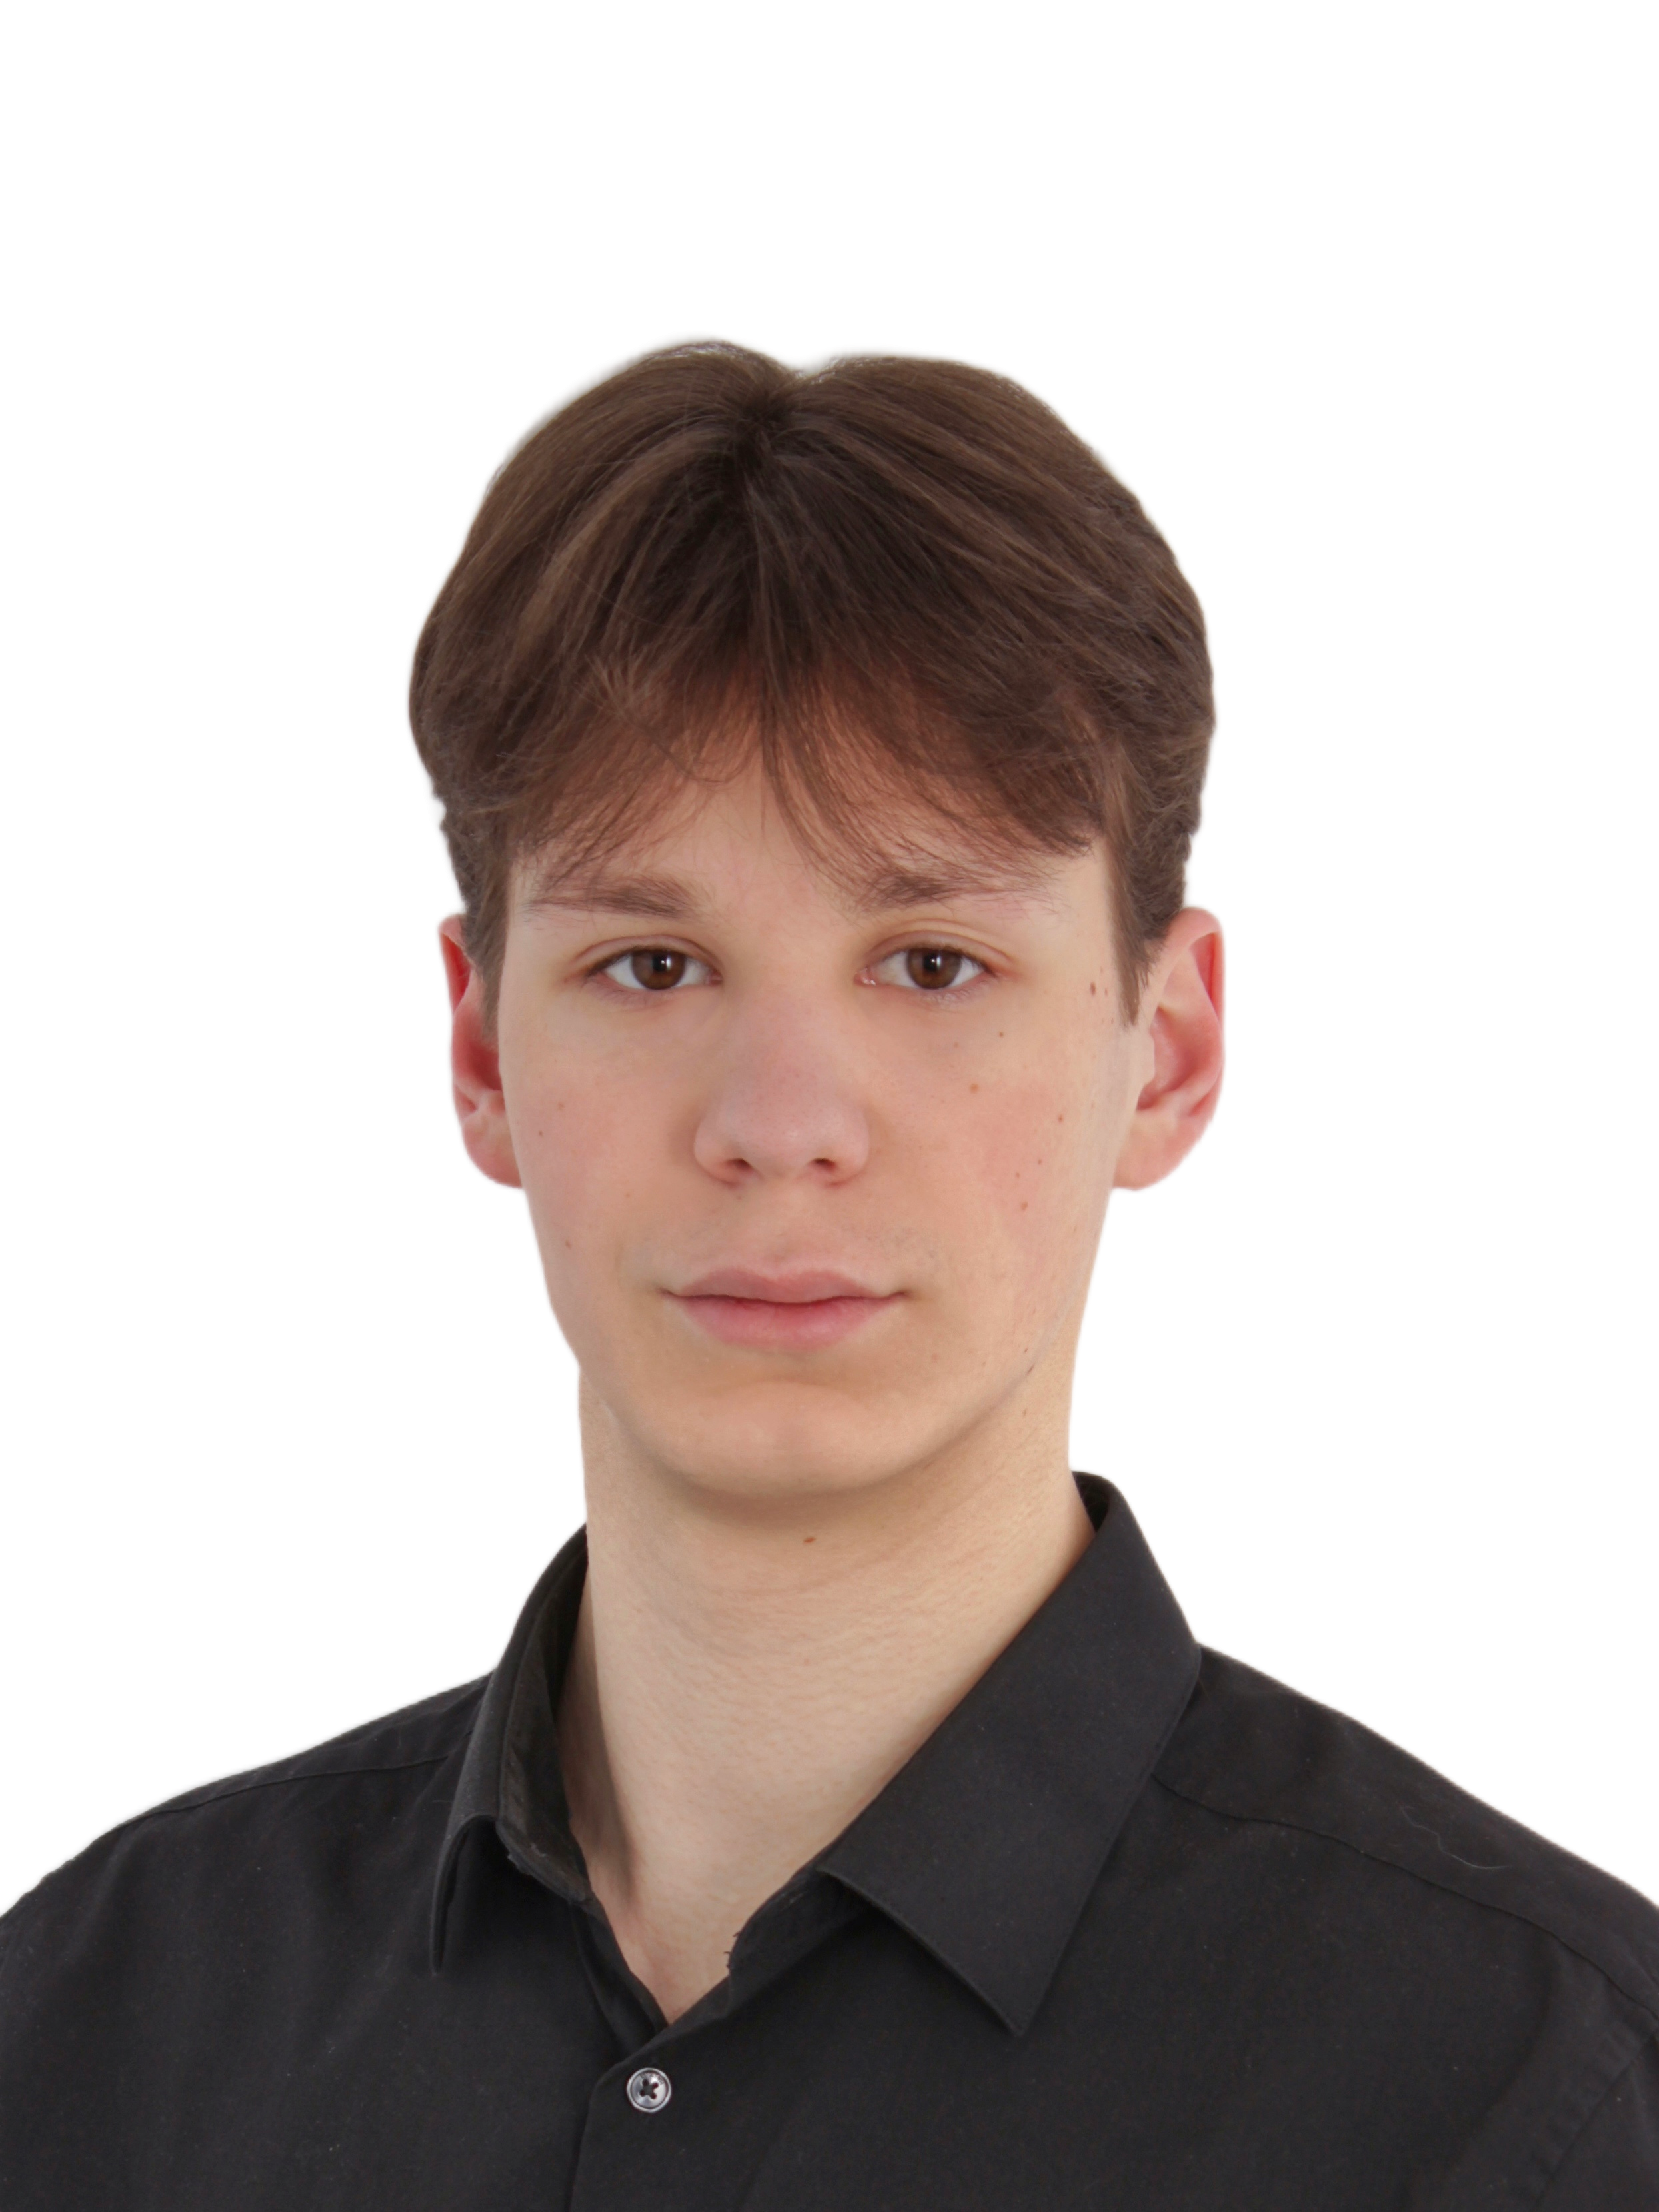
\includegraphics[width=5cm]{common/CV_Photo.png}
\end{tikzpicture}
\end{minipage}
}
\begin{minipage}[t]{0.68\textwidth}
    \cvsect{Developer}
	\vspace{-6pt}
 
    \textbf{Results-driven} MIPT student and C developer with knowledge of x86-64 assembly and basics of Python. I'm focused on \textbf{improving my C++} programming skills and expanding my computer science knowledge. I am particularly interested in projects involving \textbf{optimizations}, \textbf{OS internals} and \textbf{artificial intelligence}.
    
    \vspace{-6pt}
    \cvsect{Skills}
    \vspace{-6pt}

    \begin{minipage}[t]{0.2\textwidth}
    \textbf{Tools:}
    \end{minipage}
    \hfill
    \begin{minipage}[t]{0.73\textwidth}
        Git, Make/CMake, Linux, Radare2, Latex, Graphviz, Doxygen
    \end{minipage}
    \vspace{2mm}
    
    \begin{minipage}[t]{0.2\textwidth}
        \textbf{Libraries:}
    \end{minipage}
    \hfill
    \begin{minipage}[t]{0.73\textwidth}
        SFML, GTK
    \end{minipage}
    \vspace{2mm}
    
    \begin{minipage}[t]{0.2\textwidth}
        \textbf{Languages:}
    \end{minipage}
    \hfill
    \begin{minipage}[t]{0.73\textwidth}
        C, Bash, x86-64 assembly (NASM), ARM64, Python
    \end{minipage}
    
\end{minipage}
\vspace{2mm}

\vspace{-10 pt}
\cvsect{Education}
\vspace{-5 pt}        
\begin{entrylist}
    \entry
		{Present}
		{Moscow Institute of Physics and Technology}
		{University | Moscow, Russia}
		{System programming and applied mathematics (undergraduate)}
\end{entrylist}

\vspace{-20 pt}
\cvsect{Projects}
\vspace{-5 pt}
\begin{entrylist}
	\entry
		{2025\\\footnotesize{in process}}
		{Mandelbrot Set}
		{\href{https://github.com/livlavr/MandelbrotSet}{github.com/livlavr/MandelbrotSet}}
		{Lab work involving comparison of different types of CPU rendering, testing with the \textit{Mandelbrot set}. Three versions were compared: basic, with \textbf{compiler optimizations}, and with direct \textbf{Arm Neon Intrinsics}.\\\texttt{C/C++}\slashsep\texttt{CMake}\slashsep\texttt{SFML}\slashsep\texttt{SIMD}}
	\entry
		{2025\\\footnotesize{finished}}
		{Printf}
        {\href{https://github.com/livlavr/Printf}{github.com/livlavr/Printf}}
		{An educational project implementing the printf function from the standard C library, supporting specifications: \textit{\%(b|c|d|o|s|u|x)}. \textbf{The aim} of this project was to work with \textbf{calling conventions}, use the \textbf{stack frame} and \textbf{function arguments} in x86-64 assembly, and \textbf{identify security vulnerabilities} of the standard printf function.\\ \texttt{x86-64 assembly}\slashsep\texttt{NASM}}
	\entry
		{2024 -- 2025\\\footnotesize{in process}}
		{Programming Language}
        {\href{https://github.com/livlavr/Language}{github.com/livlavr/Language}}
		{Implementation of my own compiled programming language. The code is first processed by \textbf{lexical analysis}, then by syntax analysis using \textbf{recursive descent}, translated into a syntax tree with a name table, and finally into an assembly file (pseudo-assembly for the \textbf{CPU Emulator}). This assembly file is processed by my own SPU. I plan to compile the program into full-fledged x86-64 assembly. The project supports cross-compilation with the SPU and languages of other group students, thanks to a common AST standard.\\ \texttt{C/C++}\slashsep\texttt{Make}\slashsep\texttt{Graphviz}}
    \entry
		{2024\\\footnotesize{finished}}
		{CPU Emulator (SPU)}
        {\href{https://github.com/livlavr/SPU}{github.com/livlavr/SPU}}
		{A virtual machine emulating the interaction between the CPU and assembly instructions (\textbf{Harvard architecture}). The project consists of two parts: an \textbf{assembler for pseudo-assembly}, which translates assembly instructions into byte code, and a \textbf{processor emulator} that processes this byte code. It also supports basic video memory operations.\\ \texttt{C}\slashsep\texttt{Make}}
\end{entrylist}

\vspace{-20 pt}
\cvsect{Accolades}
\vspace{-5 pt}
\begin{entrylist}
	\entry
		{2025}
		{Rosatom Industry Mathematics Olympiad}
        {}
		{1st degree diploma}
    \entry
		{2024}
		{Computer Security I.Y. Verchenko Interregional Olympiad}
        {}
		{2st degree diploma}
\end{entrylist}

\vspace{-20 pt}
	\cvsect{Languages}
    \vspace{-6pt}
    
    \hspace{26mm} \textbf{English} - B2, \textbf{ Russian} - native

\end{document}

